\documentclass[../main.tex]{subfiles}
\graphicspath{{\subfix{../Images/}}}

\begin{document}

\chapter{Chapter 8. Bump Mapping}

This chapter enhances the per-fragment lighting discussion in Chapter 5 with texture-encoded normals to create an effect known as bump mapping. This chapter has the following five sections:

\begin{itemize}
\item \textbf{"Bump Mapping a Brick Wall"} introduces bump mapping of a single rectangle.
\item \textbf{"Bump Mapping a Brick Floor"} explains how to make bump mapping consistent for two planes.
\item \textbf{"Bump Mapping a Torus"} shows how to bump map curved surfaces that have mathematical representations, such as the torus.
\item \textbf{"Bump Mapping Textured Polygonal Meshes"} shows how to apply bump mapping to textured polygonal models.
\item \textbf{"Combining Bump Mapping with Other Effects"} combines bump mapping techniques with other textures, such as decals and gloss maps, for more sophisticated shading.
\end{itemize}

\section{8.1 Bump Mapping a Brick Wall}

The earlier presentation of lighting in Chapter 5 discussed per-vertex and per-fragment light computations. This chapter introduces an advanced lighting approach commonly called \textit{bump mapping}. Bump mapping combines per-fragment lighting with surface normal perturbations supplied by a texture, in order to simulate lighting interactions on bumpy surfaces. This effect is achieved without requiring excessive geometric tessellation of the surface.

As an example, you can use bump mapping to make surfaces appear as if they have bricks protruding from them, and mortar between the bricks.

Most real-world surfaces such as brick walls or cobblestones have small-scale bumpy features that are too fine to represent with highly tessellated geometry. There are two reasons to avoid representing this kind of fine detail using geometry. The first is that representing the model with sufficient geometric detail to capture the bumpy nature of the surface would be too large and cumbersome for interactive rendering. The second is that the surface features may well be smaller than the size of a pixel, meaning that the rasterizer could not accurately render the full geometric detail.

With bump mapping, you can capture the detailed surface features that influence an object's lit appearance in a texture instead of actually increasing the object's geometric complexity. Done well, bump mapping convinces viewers that a bump-mapped scene has more geometry and surface richness than is actually present. Bump mapping is most compelling when lights move in relation to a surface, affecting the bump-mapped surface's illuminated appearance.

Benefits of bump mapping include:

\begin{itemize}
\item A higher level of visual complexity in a scene, without adding more geometry.
\item Simplified content authoring, because you can encode surface detail in textures as opposed to requiring artists to design highly detailed 3D models.
\item The ability to apply different bump maps to different instances of the same model to give each instance a distinct surface appearance. For example, a building model could be rendered once with a brick bump map and a second time with a stucco bump map.
\end{itemize}

\subsection{8.1.1 The Brick Wall Normal Map}

Consider a wall made of bricks of varying texture stacked on top of each other in a regular pattern. Between the bricks is mortar that holds the bricks together. The mortar is set into the wall. Though a brick wall may look flat from a distance, on closer inspection, the brickwork pattern is not flat at all. When the wall is illuminated, the gaps between bricks, cracks, and other features of the brick surface scatter light quite differently than a truly flat surface.

One approach to rendering a brick wall would be to model every brick, mortar gap, and even individual cracks in the wall with polygons, each with varying surface normals used for lighting. During lighting, the surface normals at each vertex would alter the illuminated surface appearance appropriately. However, this approach may require a tremendous number of polygons.

At a sufficiently coarse scale, a brick wall is more or less flat. Aside from all the surface variations that we've mentioned, a wall's geometry is quite simple. A single rectangle can adequately represent a roughly flat rectangular section of brick wall.

\subsection{8.1.2 Storing Bump Maps As Normal Map Textures}

Before you encounter your first Cg program that lights surfaces with bump mapping, you should understand how textures for bump mapping are created and what they represent.

\subsection*{Conventional Color Textures}

Conventional textures typically contain RGB or RGBA color values, though other formats are also available. As you know, each texel in an RGB texture consists of three components, one each for red, green, and blue. Each component is typically a single unsigned byte.

Because programmable GPUs allow arbitrary math and other operations to be performed on the results of texture lookups, you can use textures to store other types of data, encoded as colors.

\subsection*{Storing Normals in Conventional Color Textures}

Bump maps can take a variety of forms. All the bump mapping examples in this book represent surface variations as surface normals. This type of bump map is commonly called a \textit{normal map}, because normals, rather than colors, are stored in the texture. Each normal is a direction vector that points away from the surface and is usually stored as a three-component vector.

Conventional RGB texture formats are typically used to store normal maps. Unlike colors that are unsigned, direction vectors require signed values. In addition to being unsigned, color values in textures are typically constrained to the [0, 1] range. Because the normals are normalized vectors, each component has a [-1, 1] range.

To allow texture-filtering hardware for unsigned colors to operate correctly, signed texture values in the [-1, 1] range are range-compressed to the unsigned [0, 1] range with a simple scale and bias.

Signed normals are range-compressed this way:

\FloatBarrier
\begin{lstlisting}
   colorComponent = 0.5 * normalComponent + 0.5;
\end{lstlisting}
\FloatBarrier

After conventional unsigned texture filtering, range-compressed normals are expanded back to their signed range this way:

\FloatBarrier
\begin{lstlisting}
   normalComponent = 2 * (colorComponent - 0.5);
\end{lstlisting}
\FloatBarrier

By using the red, green, and blue components of an RGB texture to store the \textit{x}, \textit{y}, and \textit{z} components of a normal, and range-compressing the signed values to the [0, 1] unsigned range, normals may be stored in RGB textures.

Recent GPUs support signed floating-point color formats, but normal maps are still often stored in unsigned color textures because existing image file formats for unsigned colors can store normal maps. Recent GPUs have no performance penalty for expanding range-compressed normals from textures. So whether you store normals in a range-compressed form (using an unsigned texture format) or use a signed texture format is up to you.

\subsection*{Generating Normal Maps from Height Fields}

Authoring normal maps raises another issue. Painting direction vectors in a computer paint program is very unintuitive. However, most normal maps are derived from what is known as a \textit{height field}. Rather than encoding vectors, a height field texture encodes the height, or elevation, of each texel. A height field stores a single unsigned component per texel rather than using three components to store a vector. Figure \ref{fig:8-1} shows an example of a brick wall height field. (See Plate \ref{fig:plate-12} in the book's center insert for a color version of the normal map.) Darker regions of the height field are lower; lighter regions are higher. Solid white bricks are smooth. Bricks with uneven coloring are bumpy. The mortar is recessed, so it is the darkest region of the height field.

\begin{figure}
    \centering
    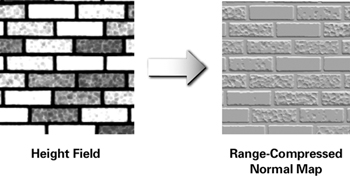
\includegraphics[width=0.75\linewidth]{fig8_1.jpg}
    \caption{Figure 8-1 A Height Field Image for a Brick Bump Map}
    \label{fig:8-1}
\end{figure}

Converting a height field to a normal map is an automatic process, and it is typically done as a preprocessing step along with range compression. For each texel in the height field, you sample the height at the given texel, as well as the texels immediately to the right of and above the given texel. The normal vector is the normalized version of the cross product of two difference vectors. The first difference vector is (1, 0, $H_a$ – $H_g$), where $H_g$ is the height of the given texel and $H_a$ is the height of the texel directly above the given texel. The second difference vector is (0, 1, $H_r$ – $H_g$), where $H_r$ is the height of the texel directly to the right of the given texel.

The cross product of these two vectors is a third vector pointing away from the height field surface. Normalizing this vector creates a normal suitable for bump mapping. The resulting normal is:

$
normal = \frac{\langle H_g - H_a, H_g - H_r, 1 \rangle}{\sqrt{(H_g - H_a)^2 + (H_g - H_r)^2 + 1}}
$

This normal is signed and must be range-compressed to be stored in an unsigned RGB texture. Other approaches exist for converting height fields to normal maps, but this approach is typically adequate.

The normal (0, 0, 1) is computed in regions of the height field that are flat. Think of the normal as a direction vector pointing up and away from the surface. In bumpy or uneven regions of the height field, an otherwise straight-up normal tilts appropriately.

As we've already mentioned, range-compressed normal maps are commonly stored in an unsigned RGB texture, where red, green, and blue correspond to \textit{x}, \textit{y}, and \textit{z}. Due to the nature of the conversion process from height field to normal map, the \textit{z} component is always positive and often either 1.0 or nearly 1.0. The \textit{z} component is stored in the blue component conventionally, and range compression converts positive \textit{z} values to the [0.5, 1] range. Thus, the predominant color of range-compressed normal maps stored in an RGB texture is blue. Figure \ref{fig:8-1} also shows the brick wall height field converted into a normal map. Because the coloration is important, you should refer to the color version of Figure \ref{fig:8-1} shown in Plate \ref{fig:plate-12}.

\subsection{8.1.3 Simple Bump Mapping for a Brick Wall}

Now that you know what a normal map is, you're ready for your first bump mapping example. The example will show how to use the brick wall normal map in Figure \ref{fig:8-1} to render a single bump-mapped rectangle to look like a brick wall. When you interactively move a single light source, you will change the appearance of the wall due to the brick pattern in the normal map, as shown in Figure \ref{fig:8-2}. The figure shows the effect of three different light positions. In the left image, the light is at the lower left of the wall. In the center image, the light is directly in front of the wall. And in the right image, the light is at the upper right of the wall.

\begin{figure}
    \centering
    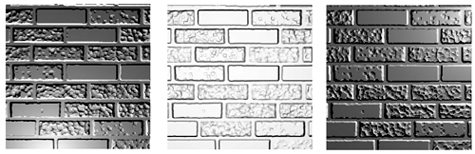
\includegraphics[width=1\linewidth]{fig8_2.jpg}
    \caption{Figure 8-2 A Bump-Mapped Brick Wall with Different Light Positions}
    \label{fig:8-2}
\end{figure}

To keep things simple, this first example is quite constrained. We position the rendered wall rectangle in the \textit{x}-\textit{y} plane, with \textit{z} equal to 0 everywhere on the wall. Without bump mapping, the surface normal for the wall would be (0, 0, 1) at every point on the wall.

\subsection*{The Vertex Program}

The \textbf{C8E1v_bumpWall} vertex program in Example 8-1 computes the object-space vector from a vertex to a single light source. The program also transforms the vertex position into clip space using a conventional modelview-projection matrix, and it passes through a 2D texture coordinate set intended to sample the normal map texture.

\FloatBarrier
\begin{lstlisting}[caption=Example 8-1. The \textbf{C8E1v_bumpWall} Vertex Program]
void  C8E1v_bumpWall(float4 position : POSITION,
                     float2 texCoord : TEXCOORD0,

                 out float4 oPosition      : POSITION,
                 out float2 oTexCoord      : TEXCOORD0,
                 out float3 lightDirection : TEXCOORD1,

             uniform float3 lightPosition, // Object space
             uniform float4x4   modelViewProj)
{
  oPosition = mul(modelViewProj, position);
  oTexCoord = texCoord;
  // Compute object-space light direction
  lightDirection = lightPosition - position.xyz;
}
\end{lstlisting}
\FloatBarrier

\subsection*{The Fragment Program}

The dot product of the light vector and the normal vector for diffuse lighting requires a unit-length light vector. Rather than implement the normalization directly with math operations, the \textbf{C8E2f_bumpSurf} fragment program in Example 8-2 normalizes the interpolated light direction vector using a \textit{normalization cube map}, which will be explained shortly. For now, think of a normalization cube map as a way to take an unnormalized vector that is interpolated as a texture coordinate set and generate a normalized and range-compressed version of it. Because the program implements normalization with a cube map texture access, this style of per-fragment vector normalization is fast and well suited for the broadest range of GPUs.

In addition to normalizing the interpolated light vector, the \textbf{C8E2f_bumpSurf} program samples the normal map with conventional 2D texture coordinates. The result of the normal map access is another range-compressed normal.

Next, the program's helper function, named \textbf{expand}, converts both the range-compressed normalized light direction and the range-compressed normal into signed vectors. Then the program computes the final fragment color with a dot product to simulate diffuse lighting.

Example 8-2 illustrates how the appearance of the brick wall changes with different light positions. The wall's surface, rendered with the \textbf{C8E1v_bumpWall} and \textbf{C8E2f_bumpSurf} programs, really looks like it has the texture of a brick wall.

\FloatBarrier
\begin{lstlisting}[caption=Example 8-2. The \textbf{C8E2f_bumpSurf} Fragment Program]
float3 expand(float3 v)
{
  return (v - 0.5) * 2; // Expand a range-compressed vector
}

void C8E2f_bumpSurf(float2 normalMapTexCoord : TEXCOORD0,
                    float3 lightDir          : TEXCOORD1,

                out float4 color : COLOR,

            uniform sampler2D normalMap,
            uniform samplerCUBE normalizeCube)

{
  // Normalizes light vector with normalization cube map
  float3 lightTex = texCUBE(normalizeCube, lightDir).xyz;
  float3 light = expand(lightTex);
  // Sample and expand the normal map texture
  float3 normalTex = tex2D(normalMap, normalMapTexCoord).xyz;
  float3 normal = expand(normalTex);
  // Compute diffuse lighting
  color = dot(normal, light);
}
\end{lstlisting}
\FloatBarrier

\subsection*{Constructing a Normalization Cube Map}

Chapter 7 explained how you could use cube maps for encoding environment maps as a way to give objects a reflective appearance. To simulate surface reflections, the 3D texture coordinate vector used for accessing the environment cube map represents a reflection vector. But cube map textures can encode other functions of direction vectors as well. Vector normalization is one such function.

The Cg Standard Library includes a routine called \textbf{normalize} for normalizing vectors. The routine has several overloaded variants, but the three-component version is most commonly used. The standard implementation of \textbf{normalize} is this:

\FloatBarrier
\begin{lstlisting}
float3  normalize(float3 v)
{
  float d = dot(v, v); // x*x + y*y + z*z
  return v / sqrt(d);
}
\end{lstlisting}
\FloatBarrier

The problem with this implementation of \textbf{normalize} is that basic fragment profiles provided by second-generation and third-generation GPUs cannot directly compile the \textbf{normalize} routine that we just presented. This is because these GPUs lack arbitrary floating-point math operations at the fragment level.

The normalization cube map—a fast way to normalize vectors supplied as texture coordinates—works on all GPUs, whether or not they support advanced fragment programmability.

\begin{framed}
Performance Tip

Even on GPUs supporting advanced fragment profiles, using normalization cube maps is often faster than implementing normalization with math operations, because GPU designers highly optimize texture accesses.
\end{framed}

Figure \ref{fig:8-3} shows how a cube map normalizes a vector. The vector (3, 1.5, 0.9) pierces the cube map on the positive \textit{x} face of the cube map, as shown. The faces of the normalization cube map are constructed such that the texel pierced by any given direction vector contains the normalized version of that vector. When signed texture components are unavailable, the normalized version of the vector may be stored range-compressed and then expanded prior to use as a normalized vector. This is what the examples in this chapter assume. So the range-compressed texel pierced by (3, 1.5, 0.9) is approximately (0.93, 0.72, 0.63). When this vector is expanded, it is (0.86, 0.43, 0.26), which is the approximate normalized version of (3, 1.5, 0.9).

\begin{figure}
    \centering
    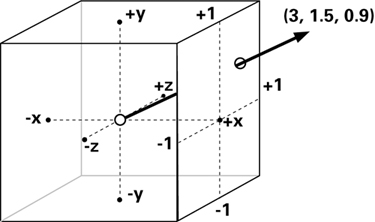
\includegraphics[width=0.75\linewidth]{fig8_3.jpg}
    \caption{Figure 8-3 Using Cube Maps to Normalize Vectors}
    \label{fig:8-3}
\end{figure}

A resolution of 32x32 texels is typically sufficient for a normalization cube map face with 8-bit color components. A resolution of 16x16, and even 8x8, can also generate acceptable results.

The electronic material accompanying this book includes a normalization cube map, as well as source code for constructing normalization cube maps. All of your Cg programs can share just one normalization cube map.

\subsection{8.1.4 Specular Bump Mapping}

You can further enhance the preceding programs by adding specular and ambient lighting terms and by adding control over the diffuse material, specular material, and light color. The next pair of programs illustrate this.

\subsection*{The Vertex Program}

Example 8-3 extends the earlier \textbf{C8E1v_bumpWall} example to compute the half-angle vector, which the rasterizer interpolates as an additional texture coordinate set. The \textbf{C8E3v_specWall} program computes the half-angle vector by normalizing the sum of the vertex's normalized light and eye vectors.

\FloatBarrier
\begin{lstlisting}[caption=Example 8-3. The C8E3v_specWall Vertex Program]
void C8E3v_specWall(float4 position : POSITION,
                    float2 texCoord : TEXCOORD0,

                out float4 oPosition      : POSITION,
                out float2 oTexCoord      : TEXCOORD0,
                out float3 lightDirection : TEXCOORD1,
                out float3 halfAngle      : TEXCOORD2,

            uniform float3 lightPosition,   // Object space
            uniform float3 eyePosition,     // Object space
            uniform float4x4 modelViewProj)
{
  oPosition = mul(modelViewProj, position);
  oTexCoord = texCoord;
  lightDirection = lightPosition - position.xyz;
  // Add the computation of a per-vertex half-angle vector
  float3 eyeDirection = eyePosition - position.xyz;
  halfAngle = normalize(normalize(lightDirection) +
                        normalize(eyeDirection));
}
\end{lstlisting}
\FloatBarrier

\subsection*{The Fragment Program}

The corresponding fragment program, shown in Example 8-4, requires more modifications. In addition to normalizing the light vector with a normalization cube map as before, the updated fragment program also normalizes the half-angle vector with a second normalization cube map. Then, the program computes the dot product of the normalized half-angle vector with the perturbed normal obtained from the normal map.

\FloatBarrier
\begin{lstlisting}[caption=Example 8-4. The \textbf{C8E4f_specSurf} Fragment Program]
float3  expand(float3  v) { return (v - 0.5) * 2; }

void C8E4f_specSurf(float2 normalMapTexCoord : TEXCOORD0,
                    float3 lightDirection    : TEXCOORD1,
                    float3 halfAngle         : TEXCOORD2,

                out float4 color : COLOR,

            uniform float  ambient,
            uniform float4 LMd, // Light-material diffuse
            uniform float4 LMs, // Light-material specular
            uniform sampler2D normalMap,
            uniform samplerCUBE normalizeCube,
            uniform samplerCUBE normalizeCube2)
{
  // Fetch and expand range-compressed normal
  float3 normalTex = tex2D(normalMap, normalMapTexCoord).xyz;
  float3 normal = expand(normalTex);
  // Fetch and expand normalized light vector
  float3 normLightDirTex = texCUBE(normalizeCube,
                                   lightDirection).xyz;
  float3 normLightDir = expand(normLightDirTex);
  // Fetch and expand normalized half-angle vector
  float3 normHalfAngleTex = texCUBE(normalizeCube2,
                                   halfAngle).xyz;
  float3 normHalfAngle = expand(normHalfAngleTex);

  // Compute diffuse and specular lighting dot products
  float diffuse = saturate(dot(normal, normLightDir));
  float specular = saturate(dot(normal, normHalfAngle));
  // Successive multiplies to raise specular to 8th power
  float specular2 = specular * specular;
  float specular4 = specular2 * specular2;
  float specular8 = specular4 * specular4;

  color = LMd * (ambient + diffuse) + LMs * specular8;
}
\end{lstlisting}
\FloatBarrier

In the original \textbf{C8E2f_bumpSurf} program, the program outputs the diffuse dot product as the final color. The final color's \textbf{COLOR} output semantic implicitly clamps any negative dot product results to zero. This clamping is required by the diffuse lighting equation, because negative illumination is physically impossible. The \textbf{C8E4f_specSurf} program combines the diffuse and specular dot products, so the program explicitly clamps negative values to zero with the \textbf{saturate} Standard Library function:

\FloatBarrier
\begin{table}
\centering
\begin{tabular}{ p{5cm} p{7cm}  } 
\hline
\textbf{saturate(x)} & Clamps a scalar or all the components of a vector to the range [0, 1]. \\
\hline
\end{tabular}
\end{table}
\FloatBarrier

Basic fragment profiles such as \textbf{fp20} and \textbf{ps_1_3} lack support for true exponentiation. To simulate specular exponentiation and support a broad range of fragment profiles, the program uses three successive multiplications to raise the specular dot product to the eighth power. Advanced profiles could use the \textbf{pow} or \textbf{lit} Standard Library functions for more generality.

Finally, the output color is computed by modulating the ambient and diffuse terms by a uniform parameter, \textbf{LMd}. The application supplies \textbf{LMd}, which represents the light color premultiplied by the material's diffuse color. Similarly, the \textbf{LMs} uniform parameter modulates the specular illumination and represents the light color premultiplied by the material's specular color.

\begin{framed}
Advanced Topic: Further Improvements

The \textbf{C8E4f_specSurf} program compiles under basic and advanced fragment profiles. Although this makes the bump mapping effect portable to a wider variety of GPUs, various improvements are possible if you target an advanced fragment profile. Following are a few examples.

\textbf{C8E4f_specSurf} binds the same normalization cube map texture into two texture units. As you saw in Chapter 7, this duplicate binding is required because basic fragment profiles can only sample a given texture unit with that texture unit's corresponding texture coordinate set. Advanced fragment profiles do not have this limitation, so a single \textbf{normalizeCube} cube map sampler can normalize both the light vector and half-angle vector.

\textbf{C8E4f_specSurf} also computes the specular exponent by raising the specular dot product to the eighth power using successive multiplies, because basic fragment profiles do not support arbitrary exponentiation. An advanced profile version could use the following code:

\FloatBarrier
\begin{lstlisting}
color = Kd * (ambient + diffuse) +
        Ks * pow(specular, specularExponent);
\end{lstlisting}
\FloatBarrier

where \textbf{specularExponent} is a uniform parameter, or even a value from a texture.

\textbf{C8E3v_specWall} computes a per-vertex half-angle vector. Ideally, you should compute the half-angle vector from the light and view vectors at every fragment. You could modify the vertex program to output the \textbf{eyeDirection} value rather than the half-angle vector. Then you could modify \textbf{C8E4f_specSurf} to compute the half-angle vector at each fragment, as shown:

\FloatBarrier
\begin{lstlisting}
   // Fetch and expand normalized eye vector
   float3 normEyeDirTex = texCUBE(normalizeCube,
                                  eyeDirection).xyz;
   float3 normEyeDir = expand(normEyeDirTex);
   // Sum light and eye vectors and normalize with cube map
   float3 normHalfAngle = texCUBE(normalizeCube,
                                  normLightDir + normEyeDir);
   normHalfAngle = expand(normHalfAngle);
\end{lstlisting}
\FloatBarrier

As explained in Chapter 5, computing the half-angle vector at every fragment creates more realistic specular highlights than computing the half-angle vector per-vertex, but it is more expensive.
\end{framed}

\subsection{8.1.5 Bump Mapping Other Geometry}

You have learned how to bump map a brick wall, and the results in Figure 8-2 are quite promising. However, bump mapping is not as simple as these first examples might have you believe.

The wall rectangle rendered in Figure 8-2 happens to be flat and has a surface normal that is uniformly (0, 0, 1). Additionally, the texture coordinates assigned to the rectangle are related to the vertex positions by a uniform linear mapping. At every point on the wall rectangle, the $s$ texture coordinate is different from the $x$ position by only a positive scale factor. The same is true of the $t$ texture coordinate and the $y$ position.

Under these considerably constrained circumstances, you can directly replace the surface normal with the normal sampled from the normal map. This is exactly what the prior examples do, and the bump mapping looks fine.

However, what happens when you bump map arbitrary geometry with the \textbf{C8E1v_bumpWall} and \textbf{C8E2f_bumpSurf} programs? What if the surface normal for the geometry is not uniformly (0, 0, 1)? What if the $s$ and $t$ texture coordinates used to access the normal map are not linearly related to the geometry's $x$ and $y$ object-space positions?

In these situations, your rendering results may resemble correct bump mapping, but a closer inspection will show that the lighting in the scene is not consistent with the actual light and eye positions. What happens is that the object-space light vector and half-angle vectors used in the per-fragment bump mapping math no longer share a consistent coordinate system with the normals in the normal map. The lighting results are therefore noticeably wrong.

\subsection*{Object-Space Bump Mapping}

One solution is to make sure that the normals stored in your normal map are oriented so that they directly replace the object-space surface normals for the geometry rendered. This means that the normal map effectively stores object-space normals, an approach known as \textit{object-space bump mapping}. This approach does work, which is why our earlier bump-mapped wall example (Figure 8-2) is correct, though only for the particular wall rectangle shown.

Unfortunately, object-space bump mapping ties your normal map textures to the specific geometry that you are bump mapping. Creating a normal map requires knowing the exact geometry to which you will apply the normal map. This means that you cannot use a single brick-pattern normal map texture to bump map all the different possible brick walls in a scene. Instead, you end up needing a different normal map for every different brick wall you render. If the object animates its object-space vertex positions, every different pose potentially requires its own object-space normal map. For these reasons, object-space bump mapping is very limiting.

\subsection*{Texture-Space Bump Mapping}

Correct bump mapping requires that the light vector and half-angle vector share a consistent coordinate system with the normal vectors in the normal map. It does not matter what coordinate system you choose, as long as you choose it consistently for all vectors in the lighting equations. Object space is one consistent coordinate system, but it is not the only choice.

You do not need to make all the normals in the normal map match up with the object-space coordinate system of the object to be bump mapped. Instead, you can rotate the object-space light vectors and half-angle vectors into the normal map's coordinate system. It is a lot less work to rotate two direction vectors into an alternative coordinate system than to adjust every normal in a normal map. The coordinate system used by the normal map texture is called \textit{texture space}, so this approach is known as \textit{texture-space bump mapping} (sometimes called \textit{tangent-space bump mapping}).

Vertex programs are efficient at transforming vectors from one coordinate system to another. The vector transformations required for texture-space bump mapping are akin to transforming positions from object space to clip space with the modelview-projection matrix.

You can program your GPU to transform each object-space light and half-angle vector into the coordinate system that matches your normal map texture.

However, a modelview-projection matrix is fixed for a given rendered object. In contrast, the transformation required to rotate object-space light and half-angle vectors into the coordinate system that matches your normal map typically varies over the surface you render. Every vertex you render may require a distinct rotation matrix!

Although it may require a distinct rotation matrix for each vertex, texture-space bump mapping has one chief advantage. It allows you to apply a single normal map texture to multiple models—or to a single model being animated—while keeping the per-fragment mathematics required for bump mapping simple and efficient enough for GPUs that support only basic fragment profiles.

\section{8.2 Bump Mapping a Brick Floor}

Before we consider bump mapping polygonal meshes, consider an only slightly more complicated case. Instead of rendering a bump-mapped brick wall that has an object-space surface normal (0, 0, 1), consider rendering the same brick-textured rectangle repositioned so it becomes a brick floor rather than a wall. The surface normal for the floor is (0, 1, 0), straight up in the $y$ direction.

In this floor example, apply the same brick normal map to the floor that you applied to the wall in the last example. However, "straight up" in the normal map is the (0, 0, 1) vector, while "straight up" for the floor in object space is (0, 1, 0). These two coordinate systems are not consistent.

What does it take to make these two coordinate systems consistent? The floor has the same normal at every point, so the following rotation matrix transforms the floor's object-space "straight up" vector to the normal map's corresponding "straight up" vector:

$
\begin{bmatrix} 0 & 0 & 1 \\ \end{bmatrix}
=
\begin{bmatrix} 0 & 1 & 0 \\ \end{bmatrix}
\begin{bmatrix} 1 & 0 & 0 \\ 0 & 0 & 1 \\ 0 & -1 & 0 \\ \end{bmatrix}
$

Sections 8.3 and 8.4 will explain the details of how to construct this 3x3 matrix for arbitrary textured rectangles and triangles. For now, the important thing is that such a matrix exists and provides a way to transform vectors from object space to the normal map's texture space.

We can use this matrix to rotate the object-space light and half-angle vectors for the floor rectangle so they match the coordinate system of the normal map. For example, if $L$ is the light vector in object space (written as a row vector), then $L'$ in the normal map coordinate system can be computed as follows:

$
L'
=
\begin{bmatrix} L_x' & L_y' & L_z' \\ \end{bmatrix}
=
\begin{bmatrix} L_x & -L_z & L_y \\ \end{bmatrix}
=
\begin{bmatrix} L_x & L_y & L_z \\ \end{bmatrix}
\begin{bmatrix} 1 & 0 & 0 \\ 0 & 0 & 1 \\ 0 & -1 & 0 \\ \end{bmatrix}
$

To perform specular texture-space bump mapping, you must also rotate the half-angle vector in object space into texture space the same way. Although this example's rotation matrix is trivial, the same principle applies to an arbitrary rotation matrix.

\subsection*{About Rotation Matrices}

You can always represent a 3D rotation as a 3x3 matrix. Each column and each row of a rotation matrix must be a unit-length vector. Moreover, each column vector is mutually orthogonal to the other two column vectors, and the same applies to the row vectors. The length of a vector transformed by a rotation matrix does not change after transformation. A 3D rotation matrix can act as the bridge between direction vectors in two 3D coordinate systems.

The columns of a rotation matrix used to transform object-space direction vectors into a normal map's texture space are named \textit{tangent (T)}, \textit{binormal (B)}, and \textit{normal (N)}, respectively. So rotation matrix entries can be labeled as in Equation 8-1.

\FloatBarrier
\begin{equationcaption}
$
\begin{bmatrix}
T_x & B_x & N_x \\
T_y & B_y & N_y \\
T_z & B_z & N_z \\
\end{bmatrix}
$
\caption{Equation 8-1 A Rotation Matrix Formed by Tangent, Binormal, and Normal Column Vectors}
\end{equationcaption}
\FloatBarrier

Given two columns (or rows) of a rotation matrix, the third column (or row) is the cross product of the two known columns (or rows). For the columns, this means that the relationship in Equation 8-2 exists.

\FloatBarrier
\begin{equationcaption}
$
B = N \times T \newline
N = T \times B \newline
T = B \times N \newline
$
\caption{Equation 8-2 Cross-Product Relationships Between Tangent, Binormal, and Normal Vectors}
\end{equationcaption}
\FloatBarrier

\subsection{8.2.1 The Vertex Program for Rendering a Brick Floor}

You can enhance the \textbf{C8E1v_bumpWall} example so that it can bump map using texture-space bump mapping. To do this, pass the tangent and normal vectors of the rotation matrix needed to transform object-space vectors into texture-space vectors.

Example 8-5's \textbf{C8E5v_bumpAny} vertex program, in conjunction with the earlier \textbf{C8E2f_bumpSurf} fragment program, can bump map the brick wall and brick floor with the same normal map texture. But to do this, you must supply the proper normal and tangent vectors of the rotation matrix that maps between object space and texture space. You must specify these two vectors for each vertex. The program computes the binormal with a cross product. Rather than requiring the binormal to be passed as yet another per-vertex parameter, the program computes the binormal in order to reduce the amount of dynamic data that the GPU must read for each vertex processed. Computing the binormal also avoids having to precompute and devote memory to storing binormals.

\FloatBarrier
\begin{lstlisting}[caption=Example 8-5. The \textbf{C8E5v_bumpAny} Vertex Program]
void C8E5v_bumpAny(float3 position : POSITION,
                   float3 normal   : NORMAL,
                   float3 tangent  : TEXCOORD1,
                   float2 texCoord : TEXCOORD0,

               out float4 oPosition      : POSITION,
               out float2 normalMapCoord : TEXCOORD0,
               out float3 lightDirection : TEXCOORD1,

           uniform float3   lightPosition,  // Object space
           uniform float3   eyePosition,    // Object space
           uniform float4x4 modelViewProj)
{
  oPosition = mul(modelViewProj, float4(position, 1));

  // Compute the object-space light vector
  lightDirection = lightPosition - position;

  // Construct object-space-to-texture-space 3x3 matrix
  float3 binormal = cross(tangent, normal);
  float3x3 rotation = float3x3(tangent,
                               binormal,
                               normal);
  // Rotate the light vector using the matrix
  lightDirection = mul(rotation, lightDirection);

  normalMapCoord = texCoord;
}
\end{lstlisting}
\FloatBarrier

Texture-space bump mapping is also known as tangent-space bump mapping because a tangent vector to the surface, in conjunction with the surface normal, establishes the required rotation matrix.

Figure \ref{fig:8-4} compares two images of a simple scene with the same bump-mapped wall and floor arrangement, the same normal map texture, the same light position, and the same \textbf{C8E2f_bumpSurf} fragment program. But each image uses a different vertex program. The lighting in the left image is consistent and correct because it uses the \textbf{C8E5v_bumpAny} vertex program with the correct object-space-to-texture-space rotation for correct texture-space bump mapping. However, the lighting in the right image is inconsistent. The lighting on the wall is correct, but the lighting on the floor is wrong. The inconsistent lighting arises because the image on the right uses the \textbf{C8E1v_bumpWall} vertex program for both the wall and the floor.

\begin{figure}
    \centering
    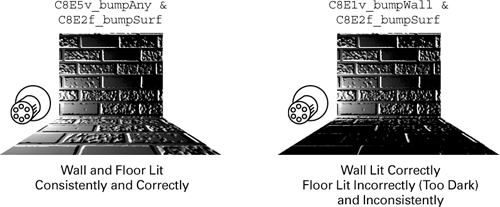
\includegraphics[width=0.75\linewidth]{fig8_4.jpg}
    \caption{Figure 8-4 Consistent Texture-Space Bump Mapping vs. Inconsistent Object-Space Bump Mapping}
    \label{fig:8-4}
\end{figure}

Conventionally, we write position vectors as column vectors and direction vectors as row vectors. Using Equation 8-2, \textbf{C8E5v_bumpAny} computes the binormal as a cross product of the per-vertex tangent and normal vectors:

\FloatBarrier
\begin{lstlisting}
float3 binormal = cross(tangent, normal);
\end{lstlisting}
\FloatBarrier

The \textbf{cross} routine for computing the cross product of two vectors is part of Cg's Standard Library.

The program then constructs a rotation matrix with the \textbf{float3x3} matrix constructor:

\FloatBarrier
\begin{lstlisting}
float3x3 rotation = float3x3(tangent,
                                binormal,
                                normal);
\end{lstlisting}
\FloatBarrier

The rows of the constructed rotation matrix are the tangent, binormal, and normal, so the constructed matrix is the transpose of the matrix shown in Equation 8-1. Multiplying a row vector by a matrix is the same as multiplying the transpose of a matrix by a column vector. The \textbf{C8E5v_bumpAny} example's multiply is a matrix-by-vector multiply because the rotation matrix is really the transpose of the intended matrix, as shown:

\FloatBarrier
\begin{lstlisting}
   lightDirection = mul(rotation, lightDirection);
\end{lstlisting}
\FloatBarrier
   
Enhancing the \textbf{C8E3v_specWall} program in the same way requires also rotating the half-angle vector, as shown:

\FloatBarrier
\begin{lstlisting}
  eyeDirection = mul(rotation, eyeDirection);
  halfAngle = normalize(normalize(lightDirection) +
                        normalize(eyeDirection));
\end{lstlisting}
\FloatBarrier

The scene in Figure \ref{fig:8-4} has only flat surfaces. This means that the rotation matrix required for the wall, and the other rotation matrix required for the floor, are uniform across each flat surface. The \textbf{C8E5v_bumpAny} program permits distinct tangent and normal vectors for every vertex. A curved surface or a mesh of polygons would require this support for varying the tangent and normal vectors that define the rotation from object space to texture space at every vertex. Figure \ref{fig:8-5} shows how a curved triangular shape requires distinct normal, tangent, and binormal vectors at each vertex. These vectors define distinct rotation matrices at each vertex that rotate the light vector properly into texture space. In the figure, the light vectors are shown in gray.

\begin{figure}
    \centering
    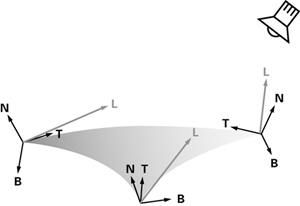
\includegraphics[width=0.5\linewidth]{fig8_5.jpg}
    \caption{Figure 8-5 Per-Vertex Texture Space Bases}
    \label{fig:8-5}
\end{figure}

The next two sections explain how to generalize texture-space bump mapping to support curved surfaces and polygonal meshes.

\section{8.3 Bump Mapping a Torus}

\begin{framed}
Advanced Topic

This section and the next are for readers who want a more mathematically based understanding of texture space. In particular, these sections explain the mathematics of how to construct the rotation matrices for transforming object-space vectors to and from texture space. These topics are not essential if you are content to rely on 3D authoring tools or other software to generate the rotation matrices for texture-space bump mapping. If you are not interested in this level of detail, you are encouraged to skip ahead to Section 8.5.
\end{framed}

In this section, we describe how to bump map a tessellated torus, as depicted in Figure \ref{fig:8-6}. Bump mapping a torus is more involved than bump mapping a brick wall because the surface of a torus curves. That curvature means that there isn't a single, fixed rotation from object space to texture space for the entire torus.

\begin{figure}
    \centering
    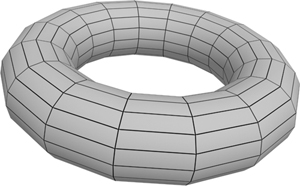
\includegraphics[width=0.75\linewidth]{fig8_6.jpg}
    \caption{Figure 8-6 A Tessellated Torus}
    \label{fig:8-6}
\end{figure}

\subsection{8.3.1 The Mathematics of the Torus}

For bump mapping, the torus provides a well-behaved surface with which to develop your mathematical intuition before you apply these ideas to the more general case of an arbitrary polygonal model in Section 8.4.

Bump mapping a torus is more straightforward than bump mapping an arbitrary polygonal model, because a single set of parametric mathematical equations, shown in Equation 8-3, defines the surface of a torus.

\FloatBarrier
\begin{equationcaption}
$
x=(M+Ncos(2\pi t))cos(2\pi s) \newline
y=(M+Ncos(2\pi t))sin(2\pi s) \newline
z=Nsin(2\pi t)
$
\caption{Equation 8-3 Parametric Equations for a Torus}
\end{equationcaption}
\FloatBarrier

The parametric variables ($s$, $t$) $\in$ [0, 1] map to 3D positions ($x$, $y$, $z$) on the torus, where $M$ is the radius from the center of the hole to the center of the torus tube, and $N$ is the radius of the tube. The torus lies in the $z=0$ plane and is centered at the origin.

By defining the surface of a torus with a set of parametric equations, you can determine the exact curvature of a torus analytically, using partial differential equations.

The analytic definition of the torus in Equation 8-3 lets you determine an oriented surface-local coordinate system, the texture space we seek for bump mapping, in terms of the parametric variables ($s$, $t$) used to define the torus. These same parametric variables also serve as texture coordinates to access a normal map texture for bump mapping.

In practical terms, this provides a way to convert an object-space light vector and an object-space view vector into a surface-local coordinate system that is consistently oriented for normals stored in a normal map texture. Once you have a set of normal, light, and view vectors in this consistent coordinate system, the lighting equations explained in Chapter 5 work correctly. As discussed in Section 8.1.5, the trick to bump mapping is finding a consistent coordinate system and properly transforming all vectors required for lighting into that space.

If we assume that a surface is reasonably tessellated, we need to compute only the light and view vectors required for lighting at each vertex, and then interpolate these vectors for computing the lighting equations for every rasterized fragment. This assumption holds well for a uniformly tessellated torus.

As with the flat brick wall, we seek a rotation, in the form of a 3 $\times$ 3 matrix, that we can use to convert object-space vectors to a surface-local coordinate system oriented according to the ($s$, $t$) parameterization of the torus. Because of the curvature of the torus, the 3 $\times$ 3 matrix must be different for every vertex of the torus.

Constructing the rotation matrices requires the partial derivatives of the parametric equations that define the torus. These are shown in Equation 8-4.

\FloatBarrier
\begin{equationcaption}
$
\frac{\delta x}{\delta s}=-2\pi (M+Ncos(2\pi t))sin(2\pi s) \newline
\frac{\delta y}{\delta s}=-2\pi (M+Ncos(2\pi t))cos(2\pi s) \newline
\frac{\delta z}{\delta s}=0 \newline
\newline
\frac{\delta x}{\delta t}=-2N\pi sin(2\pi t)cos(2\pi s) \newline
\frac{\delta y}{\delta t}=-2N\pi cos(2\pi t)sin(2\pi s) \newline
\frac{\delta z}{\delta t}=2N\pi cos(2\pi t) \newline
$
\caption{Equation 8-4 Partial Derivatives of the Parametric Torus}
\end{equationcaption}
\FloatBarrier

We call the three-component vector formed from the partial derivatives in terms of either $s$ or $t$ an \textit{inverse gradient} because it resembles the per-component reciprocal of a conventional gradient. An inverse gradient indicates the instantaneous direction and magnitude of change in surface position in terms of a single parametric variable.

You can use these inverse gradients to define a surface-local coordinate system. Forming a 3D coordinate system takes two orthogonal vectors. One vector that is essential for any surface-local coordinate system is the surface normal. By definition, the surface normal points away from the surface. You can construct the surface normal at a point on a surface by computing the cross product of two noncoincident inverse gradients to the surface at that point.

For our torus example, the surface normal $N$ is given by Equation 8-5.

\FloatBarrier
\begin{equationcaption}
$
N=\langle \frac{\delta x}{\delta s},\frac{\delta y}{\delta s},\frac{\delta z}{\delta s}\rangle \times \langle \frac{\delta x}{\delta t},\frac{\delta y}{\delta t},\frac{\delta z}{\delta t}\rangle
$
\caption{Equation 8-5 The Normal of a Surface Expressed in Terms of Its Parametric Inverse Gradients}
\end{equationcaption}
\FloatBarrier

By picking the inverse gradient in terms of s as your tangent vector, in conjunction with the surface normal, you fashion a surface-local coordinate system.

The rotation matrix required to transform object-space vectors into the texture-space coordinate system for any particular torus vertex is

\FloatBarrier
\begin{equationcaption}
$
\begin{bmatrix}
\hat{T_x} & \hat{B_x} & \hat{N_x} \\
\hat{T_y} & \hat{B_y} & \hat{N_y} \\
\hat{T_z} & \hat{B_z} & \hat{N_z} \\
\end{bmatrix}
$
\caption{Equation 8-5 The Normal of a Surface Expressed in Terms of Its Parametric Inverse Gradients}
\end{equationcaption}
\FloatBarrier

where the $\hat{V}$ notation indicates a normalized vector, and given the equations shown in Equation 8-6.

\FloatBarrier
\begin{equationcaption}
$
T=\langle \frac{\delta x}{\delta s},\frac{\delta y}{\delta s},\frac{\delta z}{\delta s}\rangle \newline
B=N\times T \newline
N=\langle \frac{\delta x}{\delta s},\frac{\delta y}{\delta s},\frac{\delta z}{\delta s}\rangle \times \langle \frac{\delta x}{\delta t},\frac{\delta y}{\delta t},\frac{\delta z}{\delta t}\rangle 
$
\caption{Equation 8-6 The Tangent, Binormal, and Normal on a Surface}
\end{equationcaption}
\FloatBarrier

You form the rotation matrix entirely of normalized vectors. This means that you can ignore the constant scale factors $2\pi$ and $2N\pi$ in Equation 8-4 for the inverse gradients in terms of $s$ and $t$, respectively.

Furthermore, the normalized surface normal $N$ of the torus based on Equation 8-5 simplifies to

$
N=\langle \cos(s)\cos(t),\sin(s)\cos(t),\sin(t)\rangle
$

\subsection{8.3.2 The Bump-Mapped Torus Vertex Program}

Example 8-6 shows the vertex program \textbf{C8E6v_torus} for rendering a bump-mapped torus. This program procedurally generates a torus from a 2D grid specified over ($s$, $t$) $\in$ [0, 1], as shown in Figure \ref{fig:8-7}. Besides generating the torus, the program constructs the correct per-vertex rotation matrix, as described in Section 8.3.1. The program also rotates the uniform object-space light vector and half-angle vector parameters into texture space for consistent texture-space bump mapping.

\begin{figure}
    \centering
    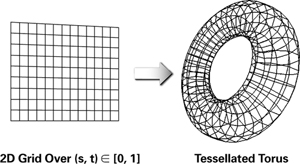
\includegraphics[width=0.75\linewidth]{fig8_7.jpg}
    \caption{Figure 8-7 Procedural Generation of a Torus from a 2D Grid}
    \label{fig:8-7}
\end{figure}

Figure \ref{fig:8-8} shows two bump-mapped tori rendered with the \textbf{C8E6v_torus} vertex program and the \textbf{C8E4f_specSurf} fragment program. The example applies the brick normal map from Figure \ref{fig:8-1}. The bricks bump outward consistently, and a specular highlight is visible in each case.

\begin{figure}
    \centering
    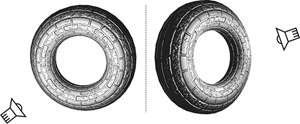
\includegraphics[width=0.75\linewidth]{fig8_8.jpg}
    \caption{Figure 8-8 Two Bump-Mapped Brick Tori Rendered with and}
    \label{fig:8-8}
\end{figure}

\FloatBarrier
\begin{lstlisting}[caption=Example 8-6. The \textbf{C8E6v_torus} Vertex Program]
void C8E6v_torus(float2 parametric : POSITION,

             out float4 position       : POSITION,
             out float2 oTexCoord      : TEXCOORD0,
             out float3 lightDirection : TEXCOORD1,
             out float3 halfAngle      : TEXCOORD2,

         uniform float3 lightPosition,  // Object space
         uniform float3 eyePosition,    // Object space
         uniform float4x4 modelViewProj,
         uniform float2 torusInfo)
{
  const float pi2 = 6.28318530;  // 2 times Pi
  // Stretch texture coordinates counterclockwise
  // over torus to repeat normal map in 6 by 2 pattern
  float M = torusInfo[0];
  float N = torusInfo[1];
  oTexCoord = parametric * float2(-6, 2);
  // Compute torus position from its parametric equation
  float cosS, sinS;
  sincos(pi2 * parametric.x, sinS, cosS);
  float cosT, sinT;
  sincos(pi2 * parametric.y, sinT, cosT);
  float3 torusPosition = float3((M + N * cosT) * cosS,
                                (M + N * cosT) * sinS,
                                N * sinT);
  position = mul(modelViewProj, float4(torusPosition, 1));
  // Compute per-vertex rotation matrix
  float3 dPds = float3(-sinS * (M + N * cosT), cosS *
                      (M + N * cosT), 0);
  float3 norm_dPds = normalize(dPds);
  float3 normal = float3(cosS * cosT, sinS * cosT, sinT);
  float3 dPdt = cross(normal, norm_dPds);
  float3x3 rotation = float3x3(norm_dPds,
                               dPdt,
                               normal);
  // Rotate object-space vectors to texture space
  float3 eyeDirection = eyePosition - torusPosition;
  lightDirection = lightPosition - torusPosition;
  lightDirection = mul(rotation, lightDirection);
  eyeDirection = mul(rotation, eyeDirection);
  halfAngle = normalize(normalize(lightDirection) +
                        normalize(eyeDirection));
}
\end{lstlisting}
\FloatBarrier

\section{8.4 Bump Mapping Textured Polygonal Meshes}

Now consider the more general case of a textured polygonal model, such as the kind used for characters and other objects in 3D computer games. In general, objects are not strictly flat like a brick wall, nor easily described with a convenient mathematical expression, like a torus. Instead, an artist models such objects as a mesh of textured triangles.

Our approach is to explain how to bump map a single triangle from a textured polygonal mesh and then generalize this method to the entire mesh.

\subsection{8.4.1 Examining a Single Triangle}

Figure \ref{fig:8-9} shows a wireframe model of an alien head, along with a height-field texture for constructing the head's normal map. The figure shows the same triangle three times. The version of the triangle on the left lies in 2D on the height-field texture. The version of the triangle on the right is shown in 3D object space in relation to other triangles forming the head. The middle version of the triangle appears on the head as rendered with bump mapping.

\begin{figure}
    \centering
    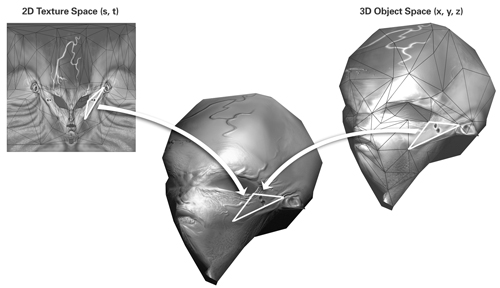
\includegraphics[width=1\linewidth]{fig8_9.jpg}
    \caption{Figure 8-9 The Same Triangle Exists in Object Space and Texture Space}
    \label{fig:8-9}
\end{figure}

Each vertex of this textured triangle has a 3D object-space position and a 2D texture coordinate set. Think of the combination of these five coordinates as a 5D vertex. You can then describe the triangle's vertices $v_0$, $v_1$, and $v_2$ this way:

\FloatBarrier
$
v_0=\langle x_0,y_0,z_0,s_0,t_0\rangle \newline
v_1=\langle x_1,y_1,z_1,s_1,t_1\rangle \newline
v_2=\langle x_2,y_2,z_2,s_2,t_2\rangle \newline
$
\FloatBarrier

Because all these coordinates lie in the plane of the same triangle, it is possible to derive plane equations for $x$, $y$, and $z$ in terms of $s$ and $t$:

\FloatBarrier
$
A_0x+B_0s+C_0t+D_0=0 \newline
A_1y+B_1s+C_1t+D_1=0 \newline
A_2z+B_2s+C_2t+D_2=0
$
\FloatBarrier

For each of these three equations, you can compute the values of the coefficients $A$, $B$, $C$, and $D$ using the triangle's vertex coordinates. For example, $A_0$, $B_0$, $C_0$, and $D_0$ would be computed as shown in Equation 8-7.

\FloatBarrier
\begin{equationcaption}
$
\langle A_0,B_0,C_0\rangle =\langle \langle x_0,s_0,t_0\rangle -\langle x_1,s_1,t_1\rangle \rangle \times \langle \langle x_0,s_0,t_0\rangle -\langle x_2,s_2,t_2\rangle \rangle \newline
D_0=-\langle A_0,B_0,C_0\rangle \cdot \langle x_0,s_0,t_0\rangle
$
\caption{Equation 8-7 Plane Equation Coefficients for (x, s, t) Plane for a Single-Textured Triangle}
\end{equationcaption}
\FloatBarrier

Rewriting the plane equations allows you to express $x$, $y$, and $z$ in terms of $s$ and $t$:

\FloatBarrier
$
x=\frac{-B_0s-C_0t-D_0}{A_0} \newline
y=\frac{-B_1s-C_1t-D_1}{A_1} \newline
z=\frac{-B_2s-C_2t-D_2}{A_2}
$
\FloatBarrier

These three equations provide a means to translate texture-space 2D positions on the triangle to their corresponding 3D positions in object space. These are simple linear functions of $s$ and $t$ that provide $x$, $y$, and $z$. The equations are similar to Equation 8-3 for the torus. As in the case of the torus, we are interested in the partial derivatives of the vector $<x, y, z>$ in terms of $s$ and $t$:

\FloatBarrier
\begin{equationcaption}
$
\langle \frac{\delta x}{\delta s},\frac{\delta y}{\delta s},\frac{\delta z}{\delta s}\rangle = \langle -\frac{B_0}{A_0},-\frac{B_1}{A_1},-\frac{B_2}{A_2}\rangle \newline
\langle \frac{\delta x}{\delta t},\frac{\delta y}{\delta t},\frac{\delta z}{\delta t}\rangle = \langle -\frac{C_0}{A_0},-\frac{C_1}{A_1},-\frac{C_2}{A_2}\rangle \newline
$
\caption{Equation 8-8 Object-Space Partial Derivatives for a Texture-Space Triangle in Terms of the Texture Coordinates}
\end{equationcaption}
\FloatBarrier

This equation provides inverse gradients analogous to those in Equation 8-4, but these inverse gradients are much simpler. Indeed, every term is a constant. That makes sense because a single triangle is uniformly flat, having none of the curvature of a torus.

Normalized versions of these inverse gradients form a rotation matrix in the same manner as the torus. Use the normalized inverse gradient in terms of $s$ as the tangent vector, and use the normalized inverse gradient in terms of $t$ as the binormal vector. You can use the cross product of these two inverse gradients as the normal vector, but if the model supplies a per-vertex normal for the vertices of the triangle, it is best to use the model's per-vertex normals instead. That's because the per-vertex normals ensure that your bump map lighting of the model is consistent with non-bump-mapped per-vertex lighting.

Normalizing the cross product of the two inverse gradients would give each triangle a uniform normal. This would create a faceted appearance.

\subsection{8.4.2 Caveats}

\subsection*{The Orthogonality of Texture Space with Object Space}

There is no guarantee that the inverse gradient in terms of $s$ will be orthogonal to the inverse gradient in terms of $t$. This happened to be true for every point on the torus (another reason the torus was used in Section 8.3), but it is not generally true. In practice, the two inverse gradients tend to be nearly orthogonal, because otherwise the artist who designed the model would have had to paint the associated texture accounting for a skew. Artists naturally choose to apply textures to models by using nearly orthogonal inverse gradients.

\subsection*{Beware of Zero-Area Triangles in Texture Space}

It is possible that two vertices of the triangle will share the same ($s$, $t$) position in texture space (or very nearly the same position), or the three texture-space positions may all be collinear. This creates a degenerate triangle with zero area in texture space (or nearly zero area). This triangle may still have area in object space; it may only be degenerate in texture space. Artists should avoid authoring such triangles if the texture coordinates are intended for bump mapping.

If zero-area triangles in texture space are present on a bump-mapped model, they have a single perturbed normal for the entire triangle, leading to inappropriate lighting.

\subsection*{Negative-Area Triangles in Texture Space}

Artists often mirror regions of a texture when applying texture coordinates to a polygonal model. For example, a texture may contain just the right half of a face. The artist can then apply the face's texture region to both the right \textit{and} the left half of the face. The same half-face image applies to both sides of the face because faces are typically symmetric. This optimization more efficiently uses the available texture resolution.

Because decals have no sense of what direction they face, this technique works fine when applying a decal texture. However, normal maps encode direction vectors that flip when polygons mirror regions of the normal map in this manner.

This issue can be avoided either by requiring artists to forgo mirroring while applying texture coordinates to models, or by automatically identifying when a triangle is mirrored in texture space and appropriately flipping the per-vertex normal direction. The latter approach is preferable, because you can use software tools to flip (negate) the normal whenever a triangle has a negative area in texture space, and adjust the mesh appropriately (for example, using NVIDIA's NVMeshMender software, which is freely available from NVIDIA's Developer Web site, \textbf{developer.nvidia.com}).

\subsection*{Nonuniform Stretching of Bump Map Texture Coordinates}

Artists can sometimes stretch a texture when assigning the texture coordinates for a model in a nonuniform manner. Again, this is usually fine for decals, but stretching creates issues for bump mapping. Nonuniform scaling of textures means that the inverse gradient in terms of $s$ may have a much larger magnitude than the inverse gradient in terms of $t$. Typically, you automatically generate normal maps from height fields without reference to a particular model. Implicitly, you are assuming that any stretching of the normal map, when it applies to the model, is uniform.

You can avoid this issue either by requiring artists to avoid nonuniform stretching, or by accounting for the stretching when converting the height-field texture to a normal map.

\subsection{8.4.3 Generalizing to a Polygonal Mesh}

You can apply the approach described in the previous section on a polygon-by-polygon basis to every polygon in your polygonal mesh. You compute the tangent, binormal, and normal for every triangle in the mesh.

\subsection*{Blending Bases at Shared Vertices}

However, in a mesh, more than one triangle may share a given vertex in the mesh. Typically, each triangle that shares a particular vertex will have its own distinct tangent, binormal, and normal vectors. Consequently, the basis—formed by the tangent, binormal, and normal vectors—for each triangle sharing the particular vertex is likewise distinct.

However, if the tangents, binormals, and normals for different triangles at a shared vertex are similar enough (and they often are), you can blend these vectors together without creating noticeable artifacts. The alternative is to create a copy of each vertex for each triangle shared by the original vertex. Generally, blending the bases at such vertices is the best approach if the vectors are not too divergent. This approach also helps to avoid a faceted appearance when a model is not optimally tessellated.

Mirroring, as discussed previously, is a situation in which the vectors are necessarily divergent. If mirroring occurs, you need to assign each triangle a distinct vertex with the appropriate tangent, binormal, and normal for each differently mirrored triangle.

\section{8.5 Combining Bump Mapping with Other Effects}

\subsection{8.5.1 Decal Maps}

The same texture coordinates used for your bump map are typically shared with decal map textures. Indeed, the discussion in Section 8.4 presumes that the texture coordinates assigned for applying a decal texture are used to derive the tangent and binormal vectors for bump mapping.

Often, when a game engine doesn't support bump mapping, artists are forced to enhance decal textures by painting lighting variations into the textures. When you bump map a surface, the bump mapping should supply these lighting variations. Artists constructing bump maps and decals must be careful to encode diffuse material variations alone, without lighting variations, in the decal map. Artists should encode geometrical surface variations in the height field from which the normal map is generated.

For example, an artist should paint a green solid shirt as solid green in the decal map. In contrast, the artist should paint the folds in the fabric of the shirt that account for the lighting variations in the height field, rather than in the decal. If artists are not careful about this, they can inadvertently create double lighting effects that make bump-mapped surfaces too dark.

\subsection{8.5.2 Gloss Maps}

It's common for some regions of an object to be shiny (such as belt buckles and armor) and other regions to be duller (such as fabric and flesh). A \textit{gloss map} texture is a type of control map that encodes how specularity varies over a model. As with the decal map and normal map, the gloss map can share the same texture coordinate parameterization with these other texture maps. The gloss map can often be stored in the alpha component of the decal map (or even the bump map), because RGBA textures are often nearly as efficient as RGB textures.

This fragment of Cg code shows how a decal texture can provide both the decal material and a gloss map:

\FloatBarrier
\begin{lstlisting}
   float4 decalTexture = tex2D(decal, texCoord);
   color = lightColor * (decal.rgb * (ambient + diffuse) +
                         decal.a   * specular);
\end{lstlisting}
\FloatBarrier

\subsection{8.5.3 Geometric Self-Shadowing}

Geometric self-shadowing accounts for the fact that a surface should not reflect a light if the light source is below the plane of the surface. For diffuse illumination, this occurs when the dot product of the light vector and the normal vector is negative. In this case, the dot product's result is clamped to zero. You can implement this in Cg as follows:

\FloatBarrier
\begin{lstlisting}
   diffuse = max(dot(normal, light), 0);
\end{lstlisting}
\FloatBarrier

Chapter 5 explained how the specular term should also account for geometric self-shadowing by clamping the specular term to zero \textit{either} when the dot product of the half-angle vector and the normal vector is negative \textit{or} when the diffuse contribution is clamped to zero. You can implement this in Cg as follows:

\FloatBarrier
\begin{lstlisting}
   specular = dot(normal, light) > 0 ?
              max(dot(normal, halfAngle), 0) : 0;
\end{lstlisting}
\FloatBarrier

When you bump map, there are actually two surface normals: the conventional interpolated normal \textit{and} the perturbed surface normal supplied by the normal map. One way to think about these two normals is that the interpolated normal is a large-scale approximation of the surface orientation, and the perturbed normal is a small-scale approximation of the surface orientation.

If \textit{either} normal faces away from the incoming light direction, then there should be no illumination from the light. When you're lighting in texture space for bump mapping, the light vector's $z$ component indicates whether the light is above or below the horizon of the geometric (or large-scale) normal. If the $z$ component is negative, the geometric orientation of the surface faces away from the light and there should be no illumination from the light on the surface. You can implement this in Cg as follows:

\FloatBarrier
\begin{lstlisting}
   diffuse = light.z > 0 ? max(dot(normal, light), 0) : 0;
\end{lstlisting}
\FloatBarrier

The \verb!?:! test enforces geometric self-shadowing for the large-scale surface orientation; the \textbf{max} function enforces geometric self-shadowing for the small-scale surface orientation. You can implement the geometric self-shadowing for specular bump mapping in Cg this way:

\FloatBarrier
\begin{lstlisting}
   specular = dot(normal, light) > 0 && light.z > 0 ?
              max(dot(normal, halfAngle), 0) : 0;
\end{lstlisting}
\FloatBarrier

Whether or not you account for geometric self-shadowing in your bump mapping is a matter of personal preference and a performance trade-off. Accounting for geometric self-shadowing caused by the large-scale surface orientation means that a light source will not illuminate some fragments that might otherwise be illuminated. However, if you do not account for geometric self-shadowing caused by the large-scale surface orientation, then lights on bump-mapped surfaces (particularly surfaces with considerable variation of surface normals) do not provide a clear cue for the direction of the incoming light.

An abrupt cut-off might cause illumination on a bump-mapped surface to flicker unnaturally because of large-scale geometric self-shadowing when the scene is animating. To avoid this problem, use a function such as \textbf{lerp} or \textbf{smoothstep} to provide a more gradual transition.

\section{8.6 Exercises}

\begin{enumerate}
\item \textbf{Try this yourself:} Use an image-editing program to replace the normal map used in Example 8-6 with a cobblestone pattern. \textit{Hint:} You can edit the file that contains the normal map. You should not need to modify any code.

\item \textbf{Try this yourself:} When generating a normal map from a height field, you can scale the difference vectors by some scalar factor \textit{s} as shown:

$
normal =\frac{<s(H_g-H_a),s(H_g-H_r),1>}{\sqrt{(s(H_g-H_a))^2+(s(H_g-H_r))^2+1}}
$

What happens visually when you regenerate a normal map from its height field with an increased value for the $s$ scale factor? What happens when you decrease the scale factor? What happens if you use one scale factor to scale $H_g-H_a$ and another scale factor to scale $H_g-H_r$?

\item \textbf{Try this yourself:} Implement bump mapping for multiple light sources by using a rendering pass per light contribution. Use "depth equal" depth testing and additive blending to combine contributions from multiple lights for a bump-mapped surface.

\section{8.7 Further Reading}

Jim Blinn invented bump mapping in 1978. Blinn's "Simulation of Wrinkled Surfaces" (ACM Press) is a seminal SIGGRAPH computer graphics paper.

Mark Peercy, John Airey, and Brian Cabral published a SIGGRAPH paper in 1997 titled "Efficient Bump Mapping Hardware" (ACM Press), which explains tangent space and its application to hardware bump mapping.

In 2000, Mark Kilgard published "A Practical and Robust Bump-Mapping Technique for Today's GPUs." The white paper explains the mathematics of bump mapping and presents a technique appropriate for third-generation GPUs. You can find this white paper on NVIDIA's Developer Web site (\textbf{developer.nvidia.com}).

Sim Dietrich published an article titled "Hardware Bump Mapping," in \textit{Game Programming Gems} (Charles River Media, 2000), that introduced the idea of using the texture coordinates of polygonal models for texture-space bump mapping.

\end{enumerate}

\end{document}